\documentclass[]{report}
\usepackage[parfill]{parskip}

\usepackage{tikz}
\usetikzlibrary{arrows.meta}

% Title Page
\title{Technisch Ontwerp Codeniacs platform}
\author{Timo Strating - medewerker bij UU-games}
\date{Februari 14, 2017, Groningen}

\renewcommand*\contentsname{Table of Content}
\pagestyle{headings}

\begin{document}
\maketitle

\tableofcontents
\newpage






\chapter{Inleiding}

Het Codeniacs platform is een interactief platform waar kinderen kunnen leren programmeren of de basis begrippen van het programmeren kunnen vinden. Het Codeniacs platform zal een centraal systeem zijn die meerdere projecten onder het Codeniacs domein versterkt en verbind. Deze opdracht is vanuit een zeer grote opdracht verkleind door de project grenzen te verleggen. De versie die opgeleverd zal gaan worden zal minder gefocust zijn op leraren en ouders en zal zich voornamelijk gaan focussen op de gebruikers / kinderen. 

\vspace{1 cm}

De belangrijkste technische aspecten van de opdracht zijn:

\begin{itemize}
	\item 2.0 versie proof
	\begin{itemize}
		\item Er moet van te voren goed zijn nagedacht over de mogelijkheid van 2.0 features.
		\newline
	\end{itemize}

	\item Groot project krappe deadline 
	\begin{itemize}
		\item Het project is relatief groot daarom worden er cutting edge technieken gebruikt om zo veel mogelijk te kunnen ontwikkelen in de ontwikkeltijd die gegeven is. Dit betekend wel dat dingen zoals security laag op het vaandel staan. Hier dient daarom de juiste balans in gevonden te worden.
		\newline
	\end{itemize} 

	\item Platform voor pc, tablet en telefoon
	\begin{itemize}
		\item Het platform zal uiteindelijk zowel op een pc als een tablet of een telefoon geoptimaliseerd te worden zodat de gebruikers (kinderen) het in zoveel mogelijk settings zouden kunnen gebruiken.
		\newline
	\end{itemize} 

	\item Centraal project binnen het Codeniacs domein
	\begin{itemize}
		\item Het platform zal als een centraal punt fungeren voor de andere projecten. Dit betekend dat de wensen van de andere project goed in kaart gebracht dienen te worden. Zodra alle wensen van alle verbonden partijen volledig in kaart zijn gebracht dienen deze ook verwerkt te worden in het design van het platform. 
		\newline
	\end{itemize}

	\item AI gids
	\begin{itemize}
		\item Het platform zal voorzien zijn van een Artificial intelligence systeem. Dit systeem zal zich voor doen als virtuele gids en zal de gebruikers door het platform heen helpen. Deze gids zal juist gebalanceerd moeten gaan worden zodat hij niet te robotachtig lijkt maar ook niet te veel tijd inneemt in het ontwikkel proces.
		\newline
	\end{itemize}

\end{itemize} 




\chapter{Klassendiagram}

\section{Inleiding}
Het project zal gebouwd worden in een programmeer taal die niet OOP first is ontworpen daarom zal er geen klassen diagram gemaakt worden vooraf de ontwikkeling.

\section{Components}
Wel zal de website worden ontwikkeld door het gebruik van components. Components zijn kleine onderdelen van de website. Hierbij moet je denken aan grote onderdelen zoals de header of de footer maar ook aan weer kleinere onderdelen zoals de profile knop in de header. Dit zijn allemaal components.

\vspace{1 cm}

De programmeer style is voor deze opdracht specifiek afgestemd. De volgende onderdelen er zijn hiervoor veel overweging naar voren gebracht. De volgende overwegingen worden gezien als de meest belangrijke.

\begin{itemize}
	\item Rapid development / toekomst uitbreidbaarheid
	\item Rapid prototyping / toekomst bestendigheid
	\item Beginnen met een boilerplate / of vanaf scratch
	\item NoSQL / SQL
	\item True isomorphic code / language specifiek domein talen voor de Database, Server en Client
\end{itemize}

Uit deze overwegingen is de keuze gemaakt om voornamelijk de linker kan van de bovenstaande tabel aan te houden in verband met de omvang van het project dat in verhouding staat tot de deadline's. 

Daarom is er gekozen om MeteorJS te gebruiken in een zeer specifieke manier. Dit wil zeggen dat het systeem zo gebouwd zal gaan worden dat code in cellen geplaatst gaan worden. Dit wordt binnen MeteorJS een component genoemd. Wordt een cel te groot of heeft het te veel verantwoordelijkheden dan zal deze worden opgesplitst in 2 of meerdere cellen. Op deze manier kan de code gemakkelijk dynamisch groter groeien.

Dit heeft wel als nadeel dat er op dit moment geen geranties zijn voor de uiteindelijke klassen structuur van het Platform. Het is daarom niet mogelijk om op dit tijdstip een overzicht te gaan geven voor de Klassen of Components die uiteindelijk gebruikt gaan worden.


\chapter{Gegevensverzameling}


\section{Database}
Alle gegevens zullen worden opgeslagen in een MongoDB database, Deze database zal op de server gaan draaien. Zodra een client de website download zal hij een kleine versie van de database downloaden en uiteindelijk gaan draaien. Dit systeem wordt een miniMongo genoemd.

De MongoDB database die als het ware uiteindelijk bij de client draait zal voor de client net doen alsof hij de enigste database is. De client kan ook alleen maar strikt met zijn eigen database communiceren. daarna gaat deze zogenoemde miniMongo database de volgende eigenschappen vertonen:

\begin{itemize}
	\item De client voert een Mongo commando uit op de database maar de database veranderd niet. Voorbeeld commando "get" oftewel haalop.
	\begin{itemize}
		\item Minimongo voert het commando uit en doet verder niks.
		\item Kan hij de data niet vinden dan controleert hij ook ff bij de server of hij de data daar wel zou mogen vergaren.
		\newline
	\end{itemize}

	\item De client voert een Mongo commando uit op de database die een aanpassing maakt op de data. Voorbeelden put, update, remove oftewel voeg iets toe, update iets of verwijder iets.
	\begin{itemize}
		\item Minimongo voert het commando uit en comminuceerd daarna terug naar de MongoDB database op de server wat veranderd is.
		\newline
	\end{itemize}

	\item De Server krijgt van een minimongo een aanpassing door voor zijn MongoDB database. Dit heeft meerder stappen en gebeurt enkel en alleen in volgende volgorde:
	\begin{enumerate}
		\item MongoDB kijkt of de het een geldig mongo commando is.
		\item MongoDB voerd het commando uit op zijn database als het commando geldig is.
		\item De MonoDb database kijkt daarna of er miniMongos zijn die hebben aangegeven dat zij de meest actuele versie willen hebben. Dit wordt gedaan door een zogenaamde subscriptie oftewel abonnement op de data. 
		\item Iedereen die een zogenaamt abonnement heeft op de data zal daarna een berichtje van de server ontvangen met daarin uitgelegd wat er is aangepast.
		\item Nadat een Client een berichtje ontvangt over zijn abonnement geeft hij dit door aan zijn eigen database oftewel zijn miniMongo.
		\item MiniMongo kijkt of de het een geldig mongo commando is.
		\item MiniMongo voerd het commando uit op zijn database als het commando geldig is.
		\item Zodra er iets in de miniMongo aangepast wordt worden de anpassingen van de database doorgegeven aan de viruele DOM.
		\item De virtuele DOM verwekt de input en veranderd de DOM zonder hem te hoeven herladen.
		\newline
	\end{enumerate}
\end{itemize}

MongoDB is een nosql database die zijn content opslaat in json achtige files. MongoDB wordt daarna door het Meteor framwork uitgebreid met een miniMongo op de client en meerdere connecties tussen de virtuele DOM, de miniMongo en de MongoDB database op de server.


\section{Gegevens opslag}
De client zal niet alleen zijn eigen database hebben maar zal ook voorzien zijn van seccion variabelen. Hierin kan een cleint gegevens opslaan die uit princiepe nooit gedeeld zouden moeten worden of opgeslagen dienen te worden. Denk hierbij aan staat een menu open ja of te nee of moeten de zoek resultaten gefilterd worden op aantal likes of op aantal weergaven.




\chapter{ERD}

%%%%%%%%%%%%%%%%%%%%%%%%%%%%%%%%%%%%%%%%%%%%%%%%%%%%%%%%%%%%%%%%%
%   http://www.texample.net/tikz/examples/android/              %
%   http://www.texample.net/tikz/examples/simple-flow-chart/    %
%%%%%%%%%%%%%%%%%%%%%%%%%%%%%%%%%%%%%%%%%%%%%%%%%%%%%%%%%%%%%%%%%
5\tikzset{ >={Latex[width=2mm,length=2mm]},
	% Specifications for style of nodes:
	base/.style = {rectangle, rounded corners, draw=black, minimum width=2.5cm, minimum height=0.75cm, text centered, font=\ttfamily},
	blue/.style = {base, fill=blue!30},
	yellow/.style = {base, fill=orange!15},
	green/.style = {base, fill=green!15},
}
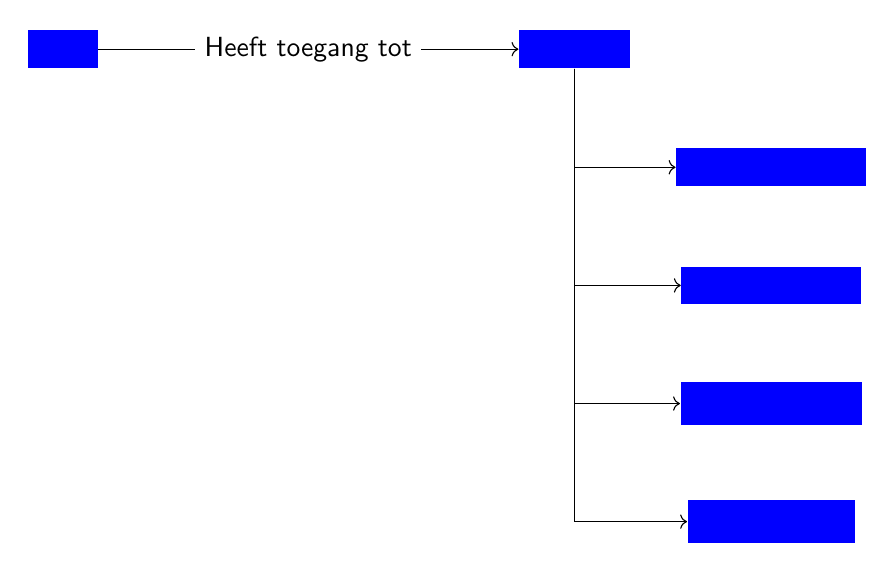
\begin{tikzpicture}[ node distance=1.5cm, every node/.style={fill=white, font=\sffamily}, align=center]
% Specification of nodes (position, etc.)

\node (user)              	[blue]              						{User};
\node (content)             [blue, right of=user, xshift=5cm]        	{Content};
\node (content-artikel)     [blue, below of=content, xshift=2.5cm]        {Content-artikel};
\node (content-video)       [blue, below of=content-artikel]        	{Content-video};
\node (content-game)        [blue, below of=content-video]        		{Content-game};
\node (content-quiz)            [blue, below of=content-game]        	{Content-quiz};

\draw[->]             (user) -- node{Heeft toegang tot}(content);
\draw[->]             (content) |- (content-artikel);
\draw[->]             (content) |- (content-video);
\draw[->]             (content) |- (content-game);
\draw[->]             (content) |- (content-quiz);

\end{tikzpicture}




\end{document}      
